\documentclass{book}
\usepackage{amsmath, amsthm, graphicx, amsfonts}
\usepackage[english]{babel}

\title{Real Time Systems for Automation\\Real Time module}
\author{Dante Piotto}
\date{Spring semester 2023}

\begin{document}

\maketitle

\chapter{Introduction}

\section{A typical control system}
%insert image from slide 17 pp1
\section{Software vision}
%inser image from slide 19
tasks share data using shared buffers

In a real time system correctness also depends on the time at which results are produced

Modularity: subsystems must be developed without knowing details about the other subsystems\\
Modularity can be achieved by: \begin{itemize}
    \item partitioning the system into a set of subsystems, each managed by one or more computational tasks
    \item defining precise interfaces between tasks, each specifying: \begin{itemize}
        \item data exchanged (I/O)
        \item function of the task
        \item validity assumptions (e.g. admissible ranges)
        \item performance requirements
    \end{itemize}
\end{itemize}
Buffers used in RTOS are tipically non blocking: \emph{Asynchronous communication mechanisms}:
\begin{itemize}
    \item Cyclic Asynchronous Buffers
    \item A message is not consumed by a receiving process but is maintained in the CAB structure until a new message is overwritten
\end{itemize}

\section{RTOS}
A RTOS is responsible for:\begin{itemize}
    \item managing cuncurrent tasks
    \item scheduling
    \item handling critical sections
    \item managing interrupts
\end{itemize}
Sources of non determinism in RT systems:
\begin{itemize}
    \item Architecture (Cache, pipelining, interrupts, DMA)
    \item OS (Scheduling, synchronization, communication)
    \item Language (lack of explicit support for time)
    \item Design methodologies: lack of analysis and verification techniques \begin{itemize}
        \item low reliability
    \end{itemize}
\end{itemize}

A RTOS requires bounded/predicable latency (controlled by architecture and choice of OS)
\subsection{Achieving predictability}
\subsubsection{DMA}
Problem: cycle stealing\\
Possible solution: time-slice method\\
each memory cycle split into two adjacent time slots, one reserved for the CPU, other oen reserved for the DMA device. Higher performance cost than cycle stealing but overall more predictable as the CPU is guaranteed half of the memory cycle
\subsubsection{Cache}
Problem: hit ratio. Preemption destroys locality. Cache related preemption delay is difficult to precisely estimate
\subsubsection{Interrupts}
Source: peripheral devices\\
Can introduce unbounded delays. ISR usually have static priorities. In generic OS I/O interrupts have real time constraints, whereas in RTOS a control process may be more urgent than interrupt handling\\
3 approaches:\begin{enumerate}
    \item Disable all interrupts except from the timer, and handle devices with polling \begin{itemize}
        \item predictable
        \item inefficient
    \end{itemize}
    \item Disable all interrupts except from the timer, and manage devices via periodic kernel routines \begin{itemize}
        \item similar to above
    \end{itemize}
    \item Leave all interrupts enabled, driver only activates device management task that gets scheduled like other tasks. \begin{itemize}
        \item no busy waiting
        \item unbounded overhead due to drivers
    \end{itemize}
\end{enumerate}
\subsubsection{System calls}
Problem: can be difficult to evaluate worst-case execution time of each task\\
Solution: system calls in RTOS should be implemented with bounded latency. Moreover, it would be desirable that system calls be preemtpable.
\subsubsection{Semaphores}
Problem: unbounded priority inversion\\
Solutions: priority inheritance, priority ceiling (Resource Access Protocols).
\subsubsection{Memory}
Problem: demand paging / page faults\\
Solution: static partitioning. Predictable, but low flexibility in dynamic environments.
\subsubsection{Programming Language}
Problems: \begin{itemize}
    \item dynamic data structures
    \item recursion
    \item cycles
\end{itemize} 
Solution: high level languages for programming hard real time applications

\chapter{Modeling Real Time Activities}
\subsubsection{Task}
 sequence of instructions that, in the absence of other activities, is continuously executed by the peocessor until completion.\\
Dispatching: Taking the first task in the ready queue and making it ready for execution
Scheduling: Deciding in which order tasks should be dispatched for execution. Decides the order of tasks in the ready queue
\\Formally: %insert def%
\subsubsection{Schedule}
Given a task set $\Gamma= \{J_1,\dots,J_n\}$, a schedule is a function $\sigma : \mathbb{R}^+ \to \mathbb{N}$ that associates an integer $k$ to each time slice $[t_i, t_{i+1} )$ with meaning: 
\begin{itemize}
    \item $k=0$: in $[t_i, t_{i+1} )$ the processor is idle
    \item $k>0$: in $[t_i, t_{i+1} )$ the processor executes $J_k$
\end{itemize}    

\subsubsection{Preemptive schedule}
Preemption is the act of suspending a running task and placing it in the ready queue
Pros:\begin{itemize}
    \item timely response to issues (exception handling)
    \item different levels of criticality: processor executes most critical tasks
    \item higher CPU utilization
\end{itemize}
Cons: \begin{itemize}
    \item introduces runtime overhead
    \item program locality is destroyed
\end{itemize}

\subsubsection{Real-Time task}
A task characterized by a timing constraint on its response time, called deadline
%insert image from slide 10
\begin{itemize}
    \item $d_i$ is the absolute deadline
    \item $D_i$ is the relative deadline
    \item The completion time is $f_i-s_i=R_i-(s_i-a_i)$
\end{itemize}
$R_i$ is the response time

\subsection{Feasibility}
%definition
\subsubsection{Feasible task}
 A Real-Time task $\tau_i$ is said to be feasible if it completes within its absolute deadline, that is, if $f_i \leq d_i$, or equivalently if $R_i \leq D_i$\\
%definition
\subsubsection{Feasible Schedule}
A schedule $\sigma$ is said to be feasible if all the tasks can complete according to a specific set of constraints
\subsubsection{Feasible task set}
A set of tasks $\Gamma$ is said to be feasible (or schedulable) if there exists at least one algorithm that can produce a feasible schedule for it.

\subsubsection{Lateness}
$L_i=f_i-d_i$\\
in a real time system lateness should be negative or at worst 0. Negative lateness is also called \emph{slack}

\subsubsection{slack time/laxity}
The difference between the relative deadline and the computation time:
\[ X_i= d_i-a_i-C_i\]
\subsubsection{tardiness/exceeding time}
\[
    E_i=max(0,L_i)
\]

\subsubsection{Job}
Instance of a task (task is a set of instructions)

\subsection{Activation mode}
\subsubsection{Time driven activation}
\begin{itemize}
    \item Periodic task, $\tau_i$
    \item the task is automatically activated by the OS at predefined time instants
    \item $a_{i,k+1}=a_{i,k}+T$
\end{itemize}
\subsubsection{Event driven activation}
\begin{itemize}
    \item Aperiodic task: job, $J_i$
    \item The task is activated at an event arrival, or by explicitly invoking a system call
    \item $a_{i,k+1}>a_{i,k}$
\end{itemize}

\subsection{Periodic task}
After completing its computation, each instance enters an idle state

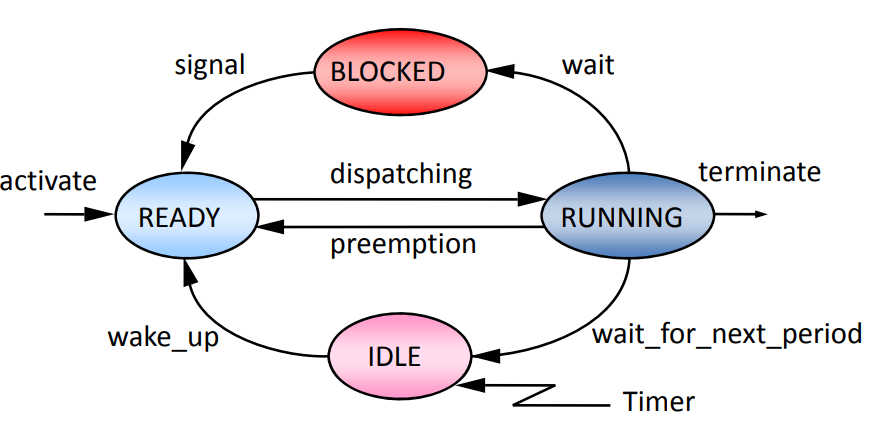
\includegraphics[width=0.9\linewidth]{images/periodictask.png}

A metascheduler is in charge of periodically waking up idle tasks. This can be done in several ways: 
\begin{itemize}
    \item using semaphores: wait/signal
    \item using message passing: blocking receive/send (QNX/neutrino)
    \item by operating on the process' state: suspend/resume (vxWorks)
\end{itemize}
The term periodic task usually means that $D_i=T_i$. If $D_i<T_i$, we call it a sporadic task
\subsubsection{Sporadic task}
A sporadic task is an aperiodic task with a \emph{minumum interarrival time} between consecutive jobs
\[a_{i,k+1} \geq a_{i,k}+T_i\]
\subsubsection{utilization factor}
 \[U_i= \frac{C_i}{T_i}\]
 in order for a task to be feasible, $U_i$ must not exceed $1$


 \chapter{Non-preemptive scheduling}
 Slide 11: ESTF= Earliest Start Time First. Differs from FCFS as it may take into consideration non shareable resources and such





\end{document}
